\section{Le fratture vertebrali}

Si tratta di fratture abbastanza frequenti: rappresentano circa il 4\% di tutte le fratture dello scheletro. Possono essere suddivise in:

\begin{itemize}
\item
  \emph{Fratture vertebrali traumatiche} che sono prevalenti tra la \emph{3\textsuperscript{o} e 4\textsuperscript{o} decade di vita} e interessano principalmente \emph{il sesso maschile}
\item
  \emph{Fratture vertebrali patologiche che colpiscono più spesso l'anziano e sono generalmente su base osteoporotica.} Queste interessano soprattutto \emph{le donne in età avanzata}. \emph{Nelle fratture vertebrali patologiche rientrano anche quelle metastatiche}
\end{itemize}


\subsection{Fratture vertebrali traumatiche}

Le fratture vertebrali \emph{traumatiche} interessano (in ordine decrescente):

\begin{itemize}
\item
  Il tratto dorso-lombare più frequentemente ed esattamente il punto di maggiore mobilità: il punto di passaggio tra la colonna toracica e la colonna lombare (T11-T12-L1)
\item
  Il tratto cervicale
\item
  Il tratto lombare
\item
  Il tratto toracico.
\end{itemize}

Le fratture vertebrali \emph{traumatiche} possono essere suddivise in:

\begin{itemize}
\item
  \textbf{FRATTURE VERTEBRALI AMIELICHE} -> Senza interessamento neurologico
\item
  \textbf{FRATTURE VERTEBRALI MIELICHE} -> Con interessamento neurologico. Sono caratterizzate da \emph{lesioni del midollo spinale} oppure \emph{delle radici nervose} che emergono dai forami di coniugazione tra una vertebra e l'altra. La gravità e l'estensione del danno neurologico dipendono dalla sede della lesione: il danno sarà tanto più severo quanto più è alta la lesione midollare quindi una lesione del rachide cervicale sarà più grave rispetto ad una lesione del tratto lombare. Fratture \emph{cervicali alte} (frattura di C1) tipo fratture \emph{del dente dell'epistrofeo} (fratture di C2 o C3) possono condurre alla \emph{morte del paziente per coinvolgimento dei centri nervosi del respiro}. Ci sono pazienti con fratture cervicali alte che oltre ad essere tetraplegici hanno anche difficoltà a respirare, a deglutire a parlare.
Nelle fratture mieliche la lesione del tessuto nervoso può essere conseguente a:
\begin{itemize}
\item
  \textbf{Compressione diretta} -> in seguito alla frattura, un frammento osseo \emph{(di un corpo vertebrale, di un arco, di un peduncolo di una vertebra)} va a schiacciare/toccare il midollo \emph{o una delle radici nervose e dà una sintomatologia periferica per:}

\begin{itemize}
\item
  \emph{Per compressione}
\item
  \emph{Per lesione (il midollo viene sezionato in parte o completamente)}
\end{itemize}

\item
  \textbf{Scivolamento di una vertebra sulla sottostante} (raro) -> si ha una lesione da taglio. \emph{Quando ad una frattura di un corpo vertebrale si associa una lussazione (cioè una dislocazione del corpo vertebrale rispetto al sottostante) ciò che sta nel mezzo viene lesionato o sezionato.} Sì immagini di avere un tubo in gomma con dentro dell'acqua: spostando la parte sottostante rispetto a quella sovrastante l'acqua uscirà sia da sopra che da sotto il tubo (lo stesso meccanismo si può avere a livello del midollo)
\item
  \textbf{Ematomielia post-traumatica} -> in seguito alla frattura si verifica un sanguinamento importante (l'osso quando si frattura sanguina molto) e si forma un ematoma che va a comprimere il midollo
\end{itemize}
\end{itemize}

\begin{figure}[!ht]
\centering
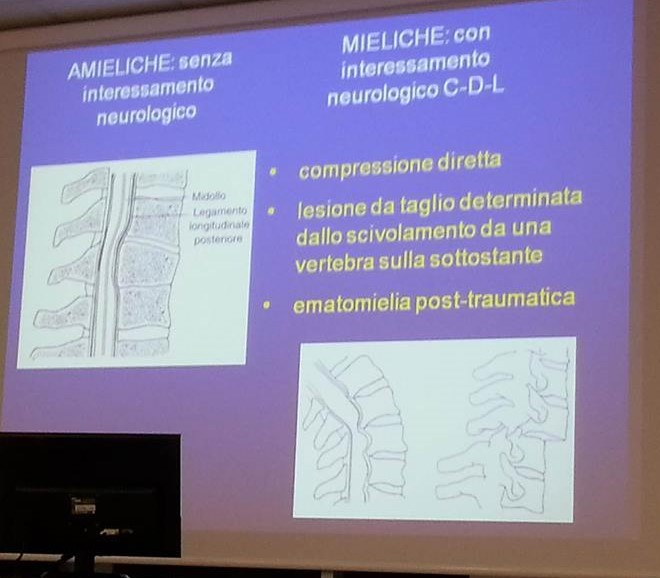
\includegraphics[width=0.5\textwidth]{003/image1.jpeg}
\end{figure}

\subsubsection{Classificazione}

Classificazione basata sul \emph{punto della vertebra} in cui queste lesioni avvengono:

\begin{itemize}
\item
  Fratture \emph{anteriori isolate} o del \emph{corpo vertebrale} (le più frequenti)
\item
  Fratture della \emph{parte posteriore} o \emph{arcali}
\item
  Fratture \emph{totali} (corpo e archi)
\item
  Fratture isolate \emph{dei peduncoli} \emph{\emph{degli archi}}, dei
  \emph{processi trasversi} o \emph{spinosi (raramente)}
\item
  \emph{Fratture-lussazioni} (casi più gravi, \emph{ma fortunatamente molto rari}): sono fratture associate ad una lussazione e quindi ad una instabilità articolare (es. spostamento di una vertebra rispetto a quella sottostante)
\item
  \emph{Fratture multiple} che interessano per esempio corpo, peduncolo, processo spinoso, processo trasverso.
\end{itemize}

\subsubsection{Clinica}

Consideriamo i due casi

\paragraph{FRATTURE VERTEBRALI AMIELICHE}

\begin{itemize}
\item
  Dolore locale in corrispondenza della zona interessata dalla frattura
\item
  Impotenza e limitazione funzionale: \emph{il paziente non riesce a piegarsi completamente sul tronco o a compiere i movimenti che normalmente e quotidianamente fa}
\item
  Alterazioni dell'atteggiamento della colonna: cifosi reattiva e/o scoliosi reattiva in vicinanza della frattura
\item
  Contrattura muscolare antalgica reattiva dei muscoli paravertebrali: \emph{per riflesso al dolore questi muscoli contraggono e determinano una \emph{scoliosi antalgica} del rachide, accompagnata dalla contrattura stessa, che è palpabile.}
\end{itemize}

\paragraph{MIELICHE CLINICA}

\begin{itemize}
\item
  Dolore locale
\item
  Impotenza e limitazione funzionale
\item
  Alterazioni dell'atteggiamento della colonna (cifosi e/o scoliosi)
\item
  Contrattura muscolare antalgica
\item
  Sintomatologia neurologica in rapporto alla sede e all'entità del trauma (37\% rachide cervicale, 22\% rachide dorsale, 8\% rachide lombare). Un paziente con una frattura mielica in T7, T8, T9, T12 avrà paraplegia (paralisi di entrambi gli arti inferiori) associata ad alterazioni sfinteriche sia delle vie urinarie che dell'apparato gastrointestinale. Un paziente che avrà una frattura mielica di C6, C7 avrà una tetraplegia (paralisi di tutti gli arti). La clinica varia a seconda del livello della lesione midollare.
\end{itemize}

\subsubsection{Diagnosi}

\paragraph{AMIELICHE/MIELICHE DIAGNOSI}

\begin{itemize}
\item
  Anamnesi
\item
  Esame obiettivo
\item
  Esami strumentali -> Radiografia, TAC, RMN, Scintigrafia
\end{itemize}

Iter in caso di trauma del rachide -> il primo passaggio è l'immobilizzazione, possibilmente in barella cucchiaio. Se si sospetta un interessamento del rachide cervicale, si deve fare indossare al paziente un collare. In PS viene fatta di base una radiografia del rachide interessato. La radiografia deve essere fatta in tutte e tre le proiezioni: anteroposteriore, latero-laterale, obliqua.
\\\\
Iter nei politraumi -> fare una TAC di tutto il rachide (senza passare attraverso la radiografia). Qualora ci sia una frattura mielica, in PS, è indicato eseguire anche una RMN che, oltre ad indicarci il danno osseo, ci permetterà di individuare la presenza e l'entità di ematomi e danni midollari dal momento che \emph{studia meglio i tessuti molli.}
\\\\
Altro punto è la valutazione dell'entità del trauma in una frattura mielinica, tale trauma potrà determinare delle condizioni più o meno reversibili:

\begin{itemize}
\item
  Commozione midollare che è sempre reversibile -> prognosi migliore. Si potrebbe fare un paragonare con il colpo del K.O nel pugilato (il sistema nervoso va in tilt per un attimo e poi si riprende).
\item
  Contusione midollare che invece non è sempre e del tutto reversibile -> quadro più grave rispetto al precedente. Il tessuto nervoso in corrispondenza della frattura ha subito una contusione cioè una sorta di trauma diretto. La RMN in questo caso può mostrare un edema del tessuto nervoso perifratturativo.
\item
  Compressione midollare che è parzialmente reversibile se dura però poche ore -> Il tessuto nervoso ha avuto un trauma diretto che persiste attraverso un meccanismo compressivo (per esempio un frammento d'osso che schiaccia il midollo oppure la presenza di un ematoma che comprime il midollo). Non c'è sezione del midollo.
\item
  Sezione midollare che è sempre irreversibile -> quadro grave in cui il midollo è stato sezionato, tagliato, distrutto. Lo stesso discorso vale per le radici nervose: quando vengono sezionate (``strappate'') non si riparano quasi mai. \emph{Discorso diverso vale per il tessuto nervoso periferico}: una lesione da taglio del nervo mediano o del nervo radiale o del nervo ulnare guarisce, soprattutto se suturata microchirurgicamente con precisione e non in tensione. I nervi periferici iniziano a rigenerare 15-20 giorni dopo la sutura: 1 mm al giorno (ricrescono in un certo senso). Di fronte ad una grossa lesione del SNP bisogna essere sempre cauti nel garantire una restitutio ad integrum della funzione del nervo.
\end{itemize}

\subsubsection{Terapia}

Il trattamento per le fratture vertebrali può essere di 2 tipi:

\begin{itemize}
\item
  \textbf{Conservativo}: impiego di busti in gesso o di tutori ortopedici che di solito nel paziente giovane devono essere tenuti per almeno tre mesi e poi abbandonati gradualmente. Questo tipo di trattamento è indicato nelle \emph{fratture stabili e amieliche}. Concetto di \textbf{stabilità}: \emph{una frattura è stabile se dal punto di vista morfologico e strutturale si è sicuri che quella frattura non si scomporrà andando a comprimente il midollo. La frattura rimarrà in quella posizione}. Una frattura amielica stabile rimarrà amielica poiché i frammenti ossei non si sposteranno e \emph{non andranno a determinare un danno nervoso}. Proprio per tale caratteristica il trattamento sarà fondamentalmente di immobilizzazione mediante busti in gesso o ortopedici. \emph{In queste fratture la sintomatologia clinica regredisce più rapidamente rispetto alla velocità con cui si vede la guarigione alle radiografie (non c'è corrispondenza tra clinica e processo di guarigione).}

\emph{Il busto va tenuto almeno 3 mesi. Di solito l'iter è:}

\begin{itemize}
\item
  \emph{Busto per 35-40 giorni}
\item
  \emph{Si toglie il busto e si fa un RX di controllo}
\item
  \emph{Si applica un altro busto di solito ortopedico per altri 40-45 giorni,}
\item
  \emph{Segue, se la radiografia va bene, un progressivo svezzamento dal busto con fisioterapia per recuperare l'articolarità del rachide.}
\end{itemize}

\emph{Nei primi giorni post-trauma per riflesso il paziente può avere un'alterazione dell'alvo e/o della diuresi: infatti prima di fare il busto dobbiamo aspettare che il paziente si canalizzi mentre per la diuresi si può mettere il catetere; si consiglia in seguito al paziente una dieta ricca di fibre.}

\item
  \textbf{Chirurgico:}

\begin{itemize}
\item
  Nel caso in cui la frattura sia \emph{amielica instabile} cioè con caratteristiche morfologiche che fanno pensare ad una possibile scomposizione della frattura e ad un possibile danno del tessuto nervoso. Si dovrà intervenire chirurgicamente andando a stabilizzare la colonna vertebrale nei giorni successivi al trauma \emph{(non in urgenza)}.
\item
  Nel caso in cui la frattura sia \emph{mielica e instabile}. In questo caso si dovrà intervenire chirurgicamente \emph{in urgenza} poiché, come visto in precedenza, ci potranno essere delle condizioni di danno nervoso potenzialmente reversibili. In questo ultimo caso, come per le fratture esposte, si pone un limite temporale tra le 6 e 8 ore dal trauma.
\end{itemize}
\end{itemize}

\begin{figure}[!ht]
\centering
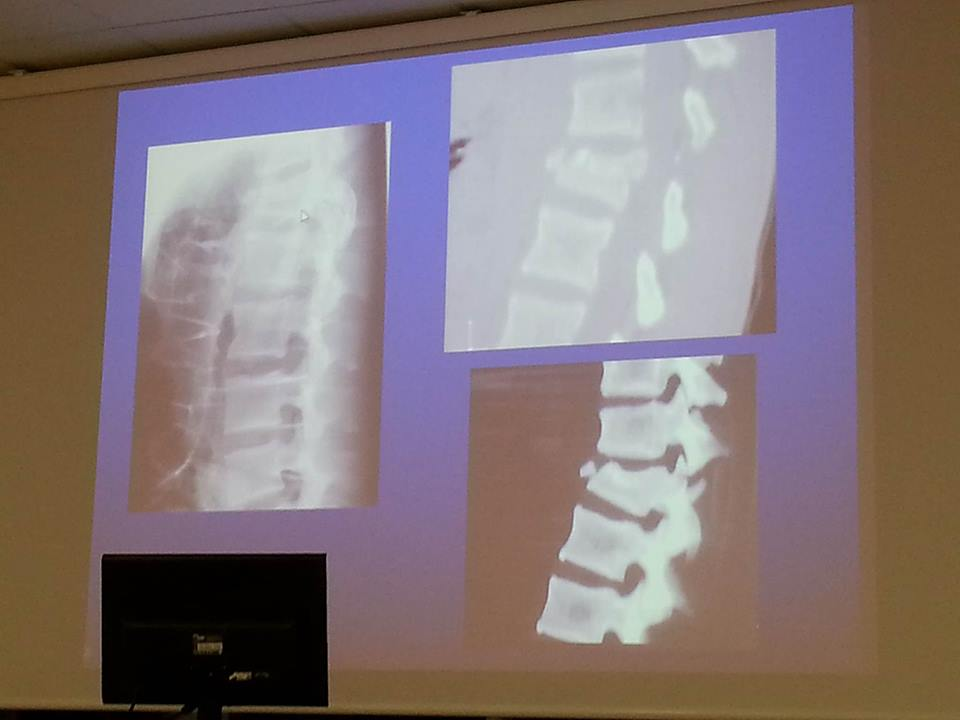
\includegraphics[width=0.7\textwidth]{003/image2.jpeg}
\end{figure}

In questa radiografia (in alto a sx) della colonna vertebrale si possono osservare corpi vertebrali normali con la tipica conformazione rettangolare e un corpo vertebrale diverso dagli altri. Quest'ultimo è
schiacciato: è deformato a cuneo. È una frattura amielica e per valutare la stabilità è stata fatta una TAC (in alto a dx) in cui si vede il corpo vertebrale fratturato che è più basso rispetto agli altri e si può
notare la presenza di un frammento osseo che protrude nel canale vertebrale con conseguente restringimento dello stesso. Ne deduciamo che questa frattura potenzialmente potrebbe diventare mielica e perciò
instabile. In questo caso è stato fatto un intervento chirurgico di riduzione e stabilizzazione con delle barre e viti peduncolari (cioè che passano attraverso i peduncoli vertebrali e vanno a fissarsi all'interno
del corpo vertebrale) che vanno messe sopra e sotto il corpo vertebrale fratturato. È stato cosi stabilizzato il corpo vertebrale lesionato.
Questo tipo di stabilizzazione nelle fratture amieliche è sufficiente mentre nelle fratture mieliche può essere indicato fare una decompressione del canale midollare: evacuazione dell'ematoma o decompressione mediante spostamento dei frammenti ossei.

\subsection{Fratture vertebrali patologiche su base osteoporotica}

Sono molto diffuse tra la popolazione anziana. A \emph{differenza} delle fratture traumatiche:

\begin{itemize}
\item
  Sono \emph{fratture vertebrali patologiche}
\item
  Colpiscono generalmente l'individuo \emph{anziano}
\item
  Sono legate \emph{a traumi di minima entità} piuttosto che ad un trauma efficiente. \emph{Molto spesso il paziente non riferisce traumi oppure ne riporta di modesti:} una banale caduta in casa, alzarsi improvvisamente dal letto
\item
  \emph{Il sesso femminile è prevalentemente interessato}.
\end{itemize}

Possiamo definirle come una sorta di \emph{cedimento strutturale} dei corpi vertebrali. Raramente sono localizzate ad un unico segmento piuttosto \emph{interessano segmenti multipli}. La \emph{deformità} evidente all'esame radiologico è definita \emph{``a cuneo'' o ``a lente biconcava''} (vedi immagina sotto)

\begin{figure}[!ht]
\centering
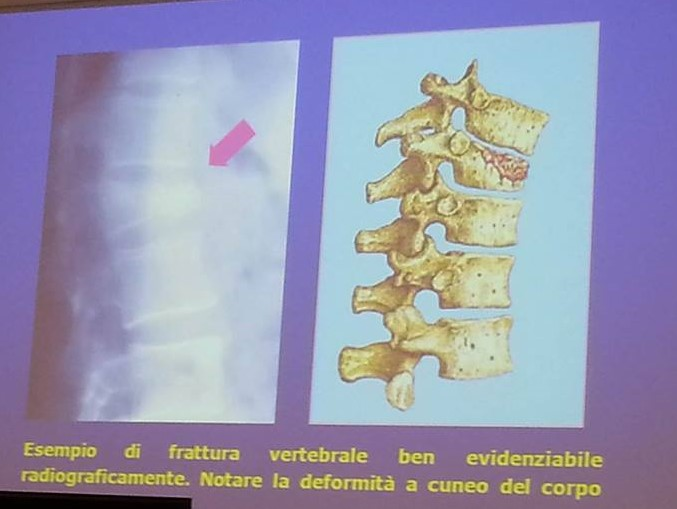
\includegraphics[width=0.7\textwidth]{003/image3.jpeg}
\end{figure}

Questo è un esempio di frattura vertebrale ben evidenziata radiograficamente. Da notare è la deformità a cuneo del corpo vertebrale

\begin{figure}[!ht]
\centering
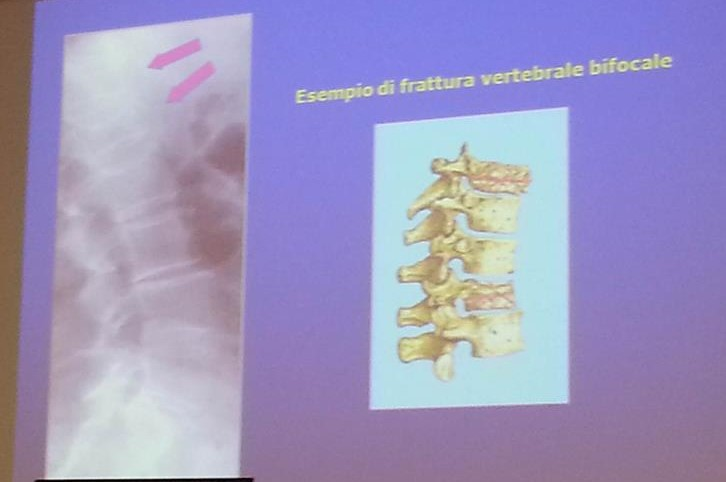
\includegraphics[width=0.7\textwidth]{003/image4.jpeg}
\end{figure}

Esempio di frattura vertebrale bifocale -> il piatto del corpo vertebrale superiormente si schiaccia e lo stesso accade per il piatto del corpo vertebrale inferiore.

\subsubsection{Clinica}

La sintomatologia nelle fratture vertebrali da osteoporosi non è particolarmente importante. Il dolore non è acuto, ma di tipo progressivo: legato al movimento, più sordo rispetto al dolore di quelle
traumatiche.

\subsubsection{Terapia}

Nella maggior parte dei casi si sceglie \emph{un trattamento incruento} e di \emph{tipo conservativo} basato sulla applicazione di busti ortopedici:

\begin{itemize}
\item
  Nel \emph{giovane} si preferiscono \emph{busti fissi metallici} per la \emph{stabilizzazione} di queste fratture
\item
  Nell'anziano affetto da comorbilità (problemi respiratori, problemi cardiovascolari, problemi addominali) si preferiscono \emph{busti in stoffa armata} (panciere di stoffa dotate di legacci e posteriormente di barre metalliche che sostengono la colonna vertebrale) fatti su misura. \emph{La scelta è dettata dal fatto che il paziente anziano non sopporta facilmente busti metallici o in gesso.} Questo tipo di trattamento ortopedico è finalizzato alla guarigione della frattura; dopodiché si cercherà di prevenire nuove fratture e il peggioramento dell'avvallamento dei corpi vertebrali attraverso una \emph{terapia sostitutiva per l'osteoporosi a base di calcio vit.D e bifosfonati.}
\end{itemize}

In \emph{alcuni casi} si potrà intervenire attraverso una \emph{metodica
più invasiva} che di solito viene eseguita dal radiologo interventista:

\begin{itemize}

\item
  \textbf{Vertebroplastica} -> introduzione attraverso \emph{una cannula}, per via percutanea (attraverso i peduncoli vertebrali nel corpo vertebrale fratturato), di metilmetacrilato (cemento acrilico) con lo scopo di aumentar la rigidità e la resistenza meccanica della vertebra al carico in compressione e \emph{nello stesso tempo alleviare il dolore}. È eseguita sotto controllo della radioscopia. Nel caso di una paziente con una vertebra osteoporotica schiacciata, datata da alcune settimane, che tende progressivamente a peggiorare e che provoca molto dolore, posso eseguire una vertebroplastica. Il cemento acrilico una volta iniettato si solidificherà e bloccherà il progressivo schiacciamento del corpo vertebrale. Come se cementassimo la colonna vertebrale.

\item
  \textbf{Cifoplastica} -> introduzione per via percutanea, attraverso i peduncoli, nel corpo vertebrale fratturato, di metimetacrilato. Come nel caso precedente però la manovra è preceduta dall' introduzione nello stesso corpo vertebrale di un palloncino espansibile che ha lo scopo di ridurre la deformità della vertebra fratturata e di creare lo spazio vuoto in cui il cemento possa penetrarvi con facilità. Attraverso il palloncino si cerca di recuperare l'altezza del corpo vertebrale fratturato mentre attraverso il cemento acrilico si cerca di mantenere questa altezza recuperata ed evitare uno schiacciamento.
\end{itemize}

\emph{La scelta tra queste due procedure sarà influenzata da:}

\begin{itemize}
\item
  \emph{Qualità ossea }
\item
  \emph{Tempistica di arrivo del paziente }
\item
  \emph{Diagnosi della frattura.}
\end{itemize}

\begin{figure}[!ht]
\centering
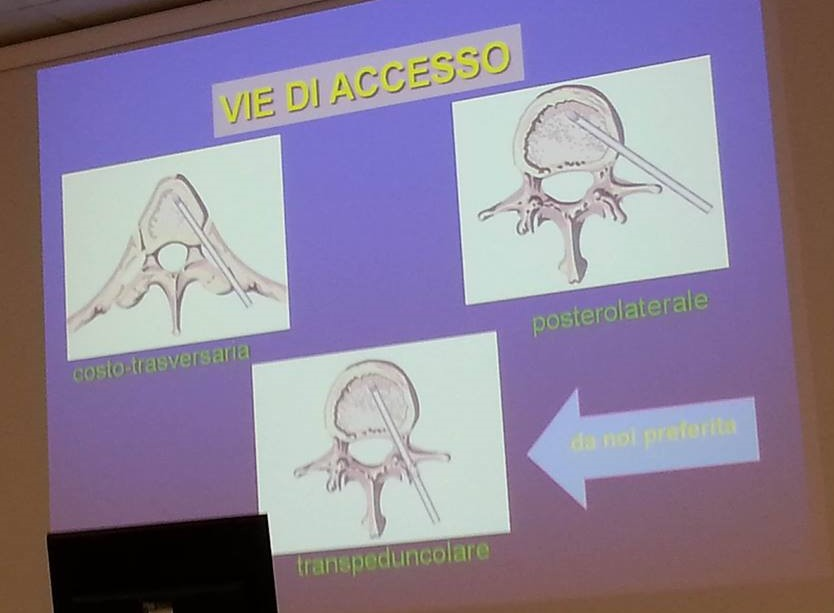
\includegraphics[width=0.7\textwidth]{003/image5.jpeg}
\end{figure}

Le due procedure di cui sopra si eseguono in sala operatoria, in anestesia peridurale o generale sotto controllo radioscopico. Quando siamo sicuri di essere all'interno del corpo vertebrale con una sorta di
cannula viene iniettato questo cemento che da prima è semiliquido e nel corso di pochi minuti diventa solido.

\begin{figure}[!ht]
\centering
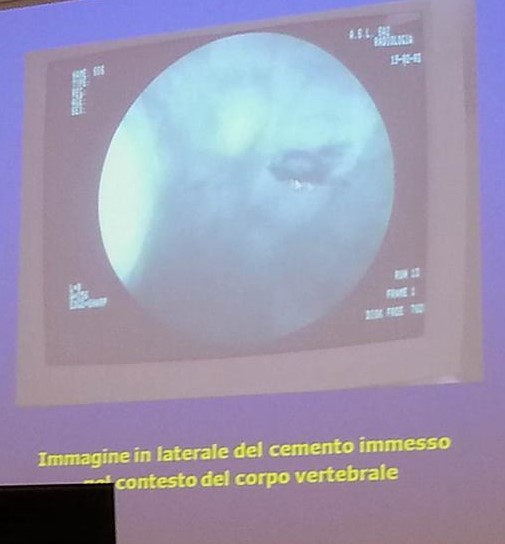
\includegraphics[width=0.7\textwidth]{003/image6.jpeg}
\end{figure}

Immagine in laterale del cemento immesso nel contesto del corpo vertebrale. Si vede una vertebra con il cemento e un'altra senza cemento.

\textbf{Complicanze vertebroplastica} -> il cemento iniettato all'interno
del corpo vertebrale potrebbe fuoriuscire nel canale vertebrale con
conseguenti:

\begin{itemize}
\item
  Danni nervosi
\item
  Danneggiamento delle strutture attorno al canale vertebrale come vasi e nervi.
\end{itemize}

Inoltre questo intervento viene eseguito in anestesia quindi ci sono tutte le complicanze legate alla sedazione. Ci sono controindicazioni per:

\begin{itemize}
\item
  Pazienti scoagulati
\item
  Pazienti con problemi cardiaci
\item
  Pazienti debilitati in generale
\end{itemize}

A volte la vertebroplastica viene eseguita \emph{in pazienti neoplastici che hanno metastasi ossee per alleviare il dolore.}

Iter riabilitativo nel paziente che ha avuto fratture ossee a causa dell'osteoporosi:

\begin{itemize}
\item
  Curare le fratture
\item
  Prevenire altre fratture attraverso la cura dell'osteoporosi
\item
  Svolgere attività fisica moderate (camminare, fare ginnastica)
\end{itemize}

\subsection{Fratture scafoide carpale e di polso}

\subsubsection{Anatomia}

Lo scafoide carpale è un osso che fa parte della prima filiera del carpo ed è chiamato scafoide o navicolare proprio perché ha la forma di una nave. È ampiamente rivestito di cartilagine ialina \emph{\emph{di tipo
articolare}} eccetto una piccola regione in cui si inseriscono i legamenti trasversi del carpo e avviene la penetrazione dei vasi ematici. \emph{Inoltre è completamente immerso all'interno del liquido
sinoviale.} Queste caratteristiche ne fanno un osso importante nella biomeccanica del carpo.
\\\\
Prima filiera del carpo -> scafoide (il più radiale), semilunare, piramidale, pisiforme
\\\\
Seconda filiera del carpo -> trapezio, trapezoide, capitato, uncinato

\begin{figure}[!ht]
\centering
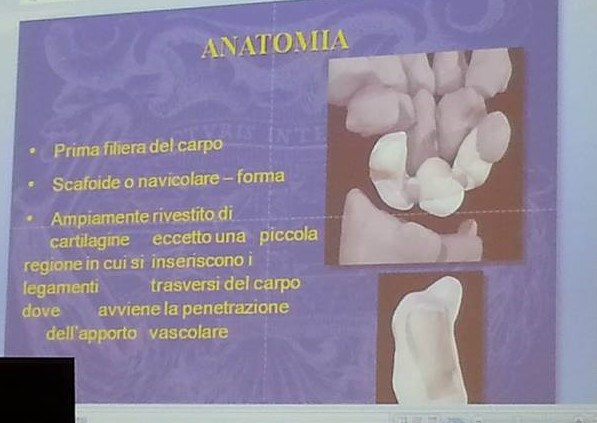
\includegraphics[width=0.7\textwidth]{003/image7.jpeg}
\end{figure}

All'osso scafoide arriva di base poco sangue e né arriverà ancora meno nel momento in cui si frattura. Inoltre ha una \emph{vascolarizzazione} di \emph{tipo terminale} (ramo dell'arteria radiale) e avviene \emph{in maniera retrograda} ossia \emph{il sangue penetra dal polo distale dello scafoide e va a vascolarizzare il polo prossimale}. Da quanto detto si
può facilmente capire perché le fratture del polo distale avranno una prognosi migliore: il \emph{sangue arriva prima e in quantità maggiore} rispetto a quelle del polo prossimale in cui il sangue arriva dopo e in
minor quantità.

\subsubsection{Epidemiologia}

\emph{Queste fratture sono più frequenti nel giovane maschio adulto:}

\begin{itemize}
\item
  \emph{In una bassa percentuale dei casi (2-3\%) sono bilaterali}
\item
  \emph{La maggior parte dei pz ha meno di 30 anni}
\item
  \emph{Viene colpito maggiormente il lato dominante}
\item
  \emph{Nell'85\% dei casi sono lesioni isolate (ossia solo fratture di scafoide)}
\item
  \emph{Nel 15\% sono associate ad altre lesioni della mano o del polso come per esempio fratture del radio associate o lesioni legamentose dei legamenti intra carpali.}
\end{itemize}

\emph{Non di rado queste fratture vengono riconosciute a distanza di 15-20-30 giorni quando la frattura non è più tale ed è diventata una \textbf{\emph{pseudoartrosi}}. Le caratteristiche generale dell'osso (vascolarizzazione, immersione nel liquido sinoviale, ritardo di calcificazione rispetto alle altre ossa) lo rendono già di base più suscettibile alla pseudoartrosi. In caso di fratture non riconosciute e trattare tempestivamente, si aggiunge un ulteriore fattore rappresentato dal trauma stesso:}

\begin{itemize}
\item
  \emph{Il liquido sinoviale si infiltra all'interno della frattura ostacolandone la guarigione}
\item
  \emph{La vascolarizzazione scarsa e di tipo terminale fa sì che, al momento della frattura, l'apporto di sangue sia facilmente insufficiente}
\item
  \emph{Lenta ossificazione}
\end{itemize}


\subsubsection{Eziopatogenesi}

\begin{figure}[!ht]
\centering
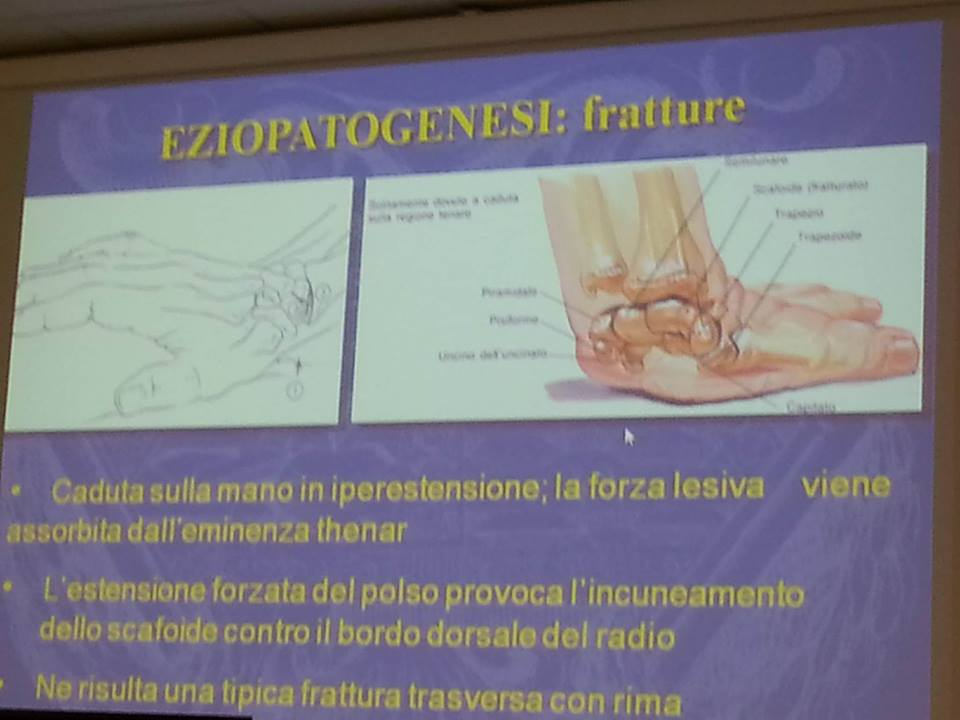
\includegraphics[width=0.7\textwidth]{003/image8.jpeg}
\end{figure}

Il trauma è di solito associato ad una caduta di media energia sul palmo della mano in iperestensione dorsale: la forza lesiva viene assorbita dall'eminenza tenar. L'estensione forzata del polso provoca l'incuneamento dello scafoide contro il bordo dorsale del radio che
funziona da leva e può rompere lo scafoide. Ne risulta una tipica frattura trasversa con rima decorrente nel terzo medio dello scafoide: la frattura ha inizio sulla superficie palmare e si propaga dorsalmente

\subsubsection{Classificazione}

\begin{figure}[!ht]
\centering
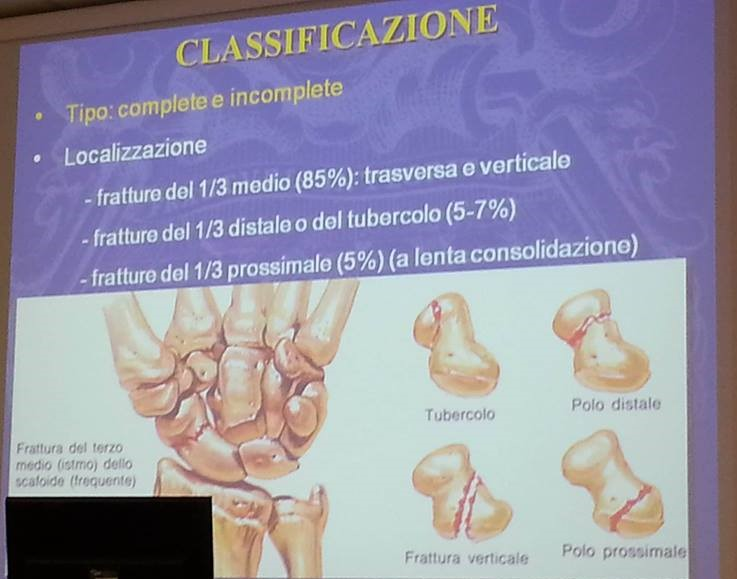
\includegraphics[width=0.7\textwidth]{003/image9.jpeg}
\end{figure}

Vengono classificate in base:

\begin{itemize}
\item
  \emph{Tipo}:
\begin{itemize}
\item[1.] \textbf{Complete}
\item[2.] \textbf{Incomplete}
\end{itemize}
\item
  \emph{Localizzazione} (è importante sapere la sede della lesione per il discorso fatto in precedenza sulla vascolarizzazione dello scafoide e perché ci dà indicazioni di tipo prognostico)
\begin{itemize}
\item[1.]
  Fratture del \textbf{1/3 medio} ovvero del \textbf{corpo dello scafoide} (85\%): trasversa (più frequente) e verticale
\item[2.]
  Fratture del \textbf{1/3 distale} o del \textbf{tubercolo} o del \textbf{polo distale} (5 \%) associate a una buona prognosi
\item[3.]
  Fratture del \textbf{1/3 prossimale} o \textbf{polo prossimale} (5\%). \emph{In questo caso entra in gioco il fattore legato alla vascolarizzazione di tipo retrogrado} da cui la prognosi peggiore e la più lenta consolidazione
\end{itemize}
\end{itemize}

\subsubsection{Diagnosi}

\begin{itemize}
\item
  Anamnesi positiva per trauma
\item
  Esame obiettivo:
\begin{itemize}
\item
  Dolore
\item
  Tumefazione della tabacchiera anatomica
\item
  Impotenza funzionale\emph{: il paziente fa fatica a muovere il polso soprattutto in alcuni tipi di movimenti cioè quelli che comportano prono-supinazione come avvitare o svitare un boccetto, chiudere la porta}
\item
  Tipico è il segno della ``o'' cioè l'esaminatore schiaccia tra pollice e indice lo scafoide e questo evoca dolore
\end{itemize}

\begin{figure}[!ht]
\centering
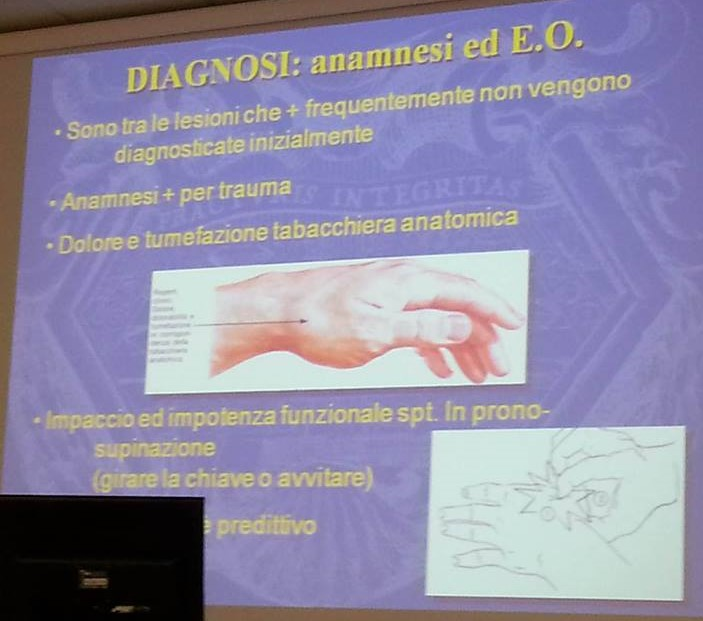
\includegraphics[width=0.7\textwidth]{003/image10.jpeg}
\end{figure}

\item
  Radiografia

\begin{itemize}
\item
  Rx del polso standard antero-posteriore e latero-laterale: non sempre permettono di fare diagnosi
\item
  Rx con proiezione specifica per lo scafoide: proiezione postero-anteriore con polso deviato ulnarmente. Questa proiezione permette la diagnosi \emph{perché il movimento di deviazione ulnare tende a diastasare, allontanare e quindi far vedere meglio un eventuale presenza di una rima di frattura a livello dello scafoide}
\end{itemize}
\end{itemize}

\begin{figure}[!ht]
\centering
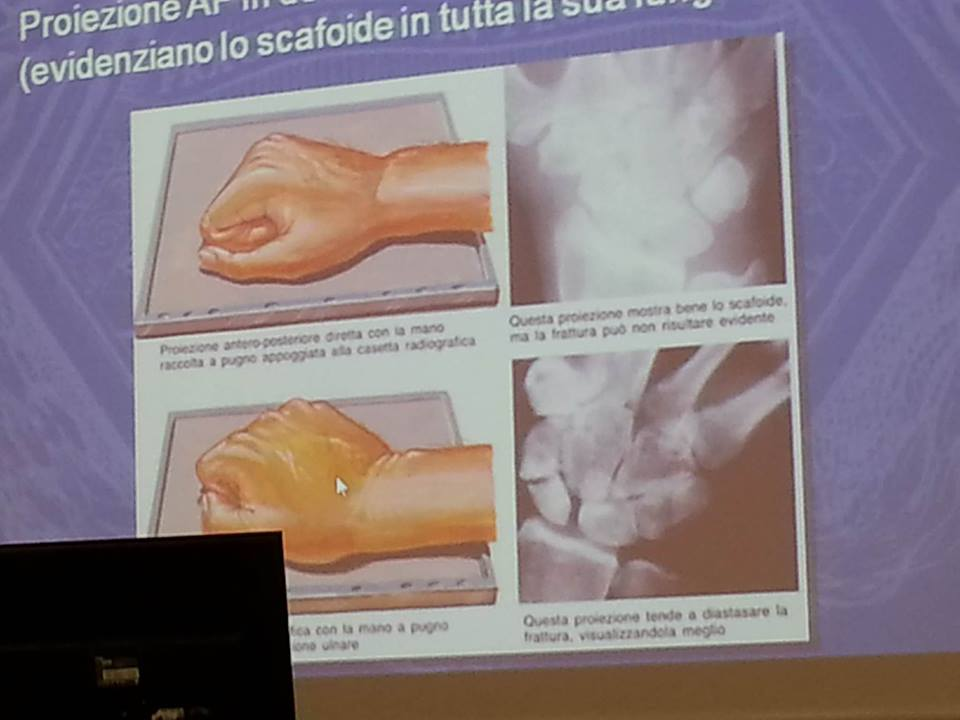
\includegraphics[width=0.7\textwidth]{003/image11.jpeg}
\end{figure}

Nella prima immagine si può vedere il polso in posizione antero-posteriore normale; nella seconda immagine si vede il polso in deviazione ulnare che tende a diastasare e a mettere in evidenza la
frattura.

NB: Molto spesso nelle prime radiografie la frattura dell'osso scafoide non si vede! \emph{Perciò se si ha un sospetto clinico importante, con dolore importate, un approccio potrebbe essere quello di \emph{immobilizzare temporaneamente l'articolazione per una settimana}}
con un tutore o con una stecca gessata. Dopo 7-10 giorni si toglie e si
fa una rivalutazione e se il paziente ha ancora dolore si procede con
un'altra radiografia o ancor meglio con una TAC con tagli specifici
sullo scafoide che nella quasi totalità dei casi mette in evidenza la
frattura. Non è raro misconoscere la frattura dello scafoide \emph{vuoi
perché il paziente tende a sottovalutare il dolore o vuoi perché a volte
gli esami non la mettono in evidenza.} In questo caso il paziente si
ripresenta dopo 4-5 mesi con un dolore cronico a livello del polso, si
fa una Rx e si mette in evidenza non più una frattura dello scafoide
bensì \emph{una pseudoartrosi dello scafoide.}
